\section{Bubble Sort}
L'idea di base è quella di scandire ripetutamente l'array dal primo all'ultimo
elemento scambiando tra loro gli elementi adiacenti che non risultino ordinati.
L'array sarà ordinato quando si riuscirà ad effettuare una scansione senza alcuno
scambio.

\begin{figure}[h]
    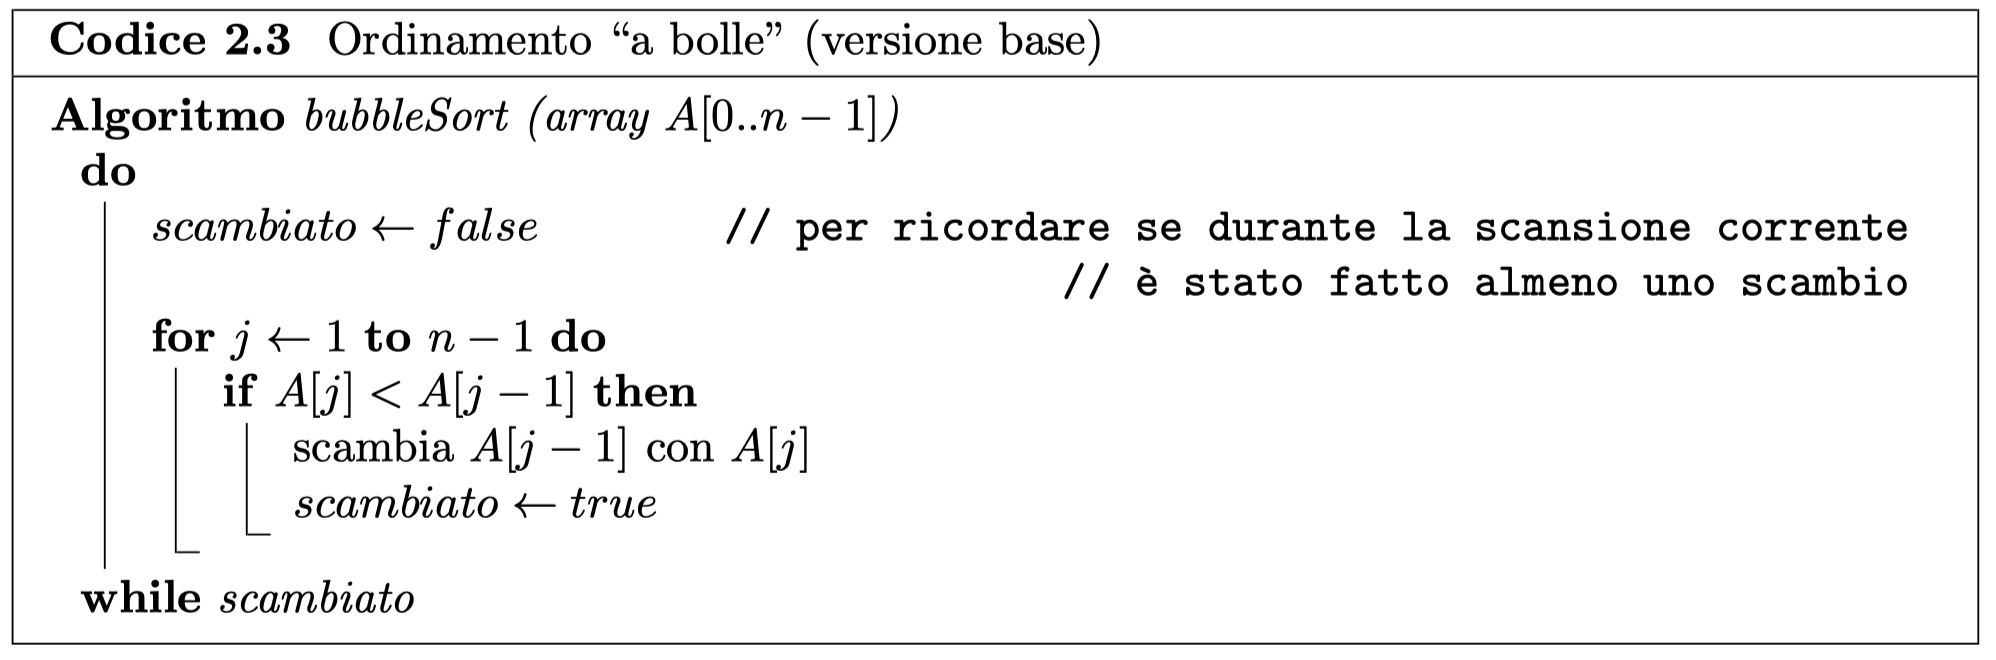
\includegraphics[width=\textwidth]{bubblesortbase.png}
\end{figure}

\subsubsection*{Esempio di esecuzione versione base}

\begin{figure}[h]
    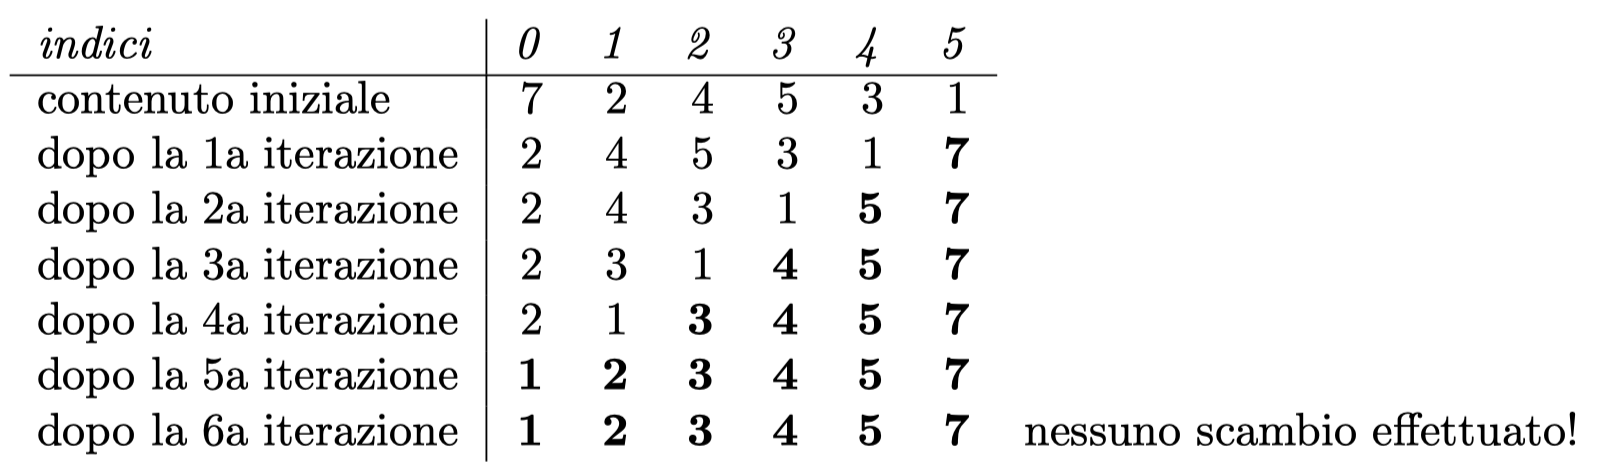
\includegraphics[width=\textwidth]{bubblesortexbase.png}
\end{figure}

\noindent Dopo la $i$-esima iterazione, gli ultimi $i$ elementi dell'array sono 
al loro posto definitivo e dunque non è più necessario esaminarli. Per la 
stessa ragione dopo $n - 1$ scansioni, gli $n - 1$ elementi più grandi hanno 
raggiunto la loro posizione e di conseguenza l'elemento più piccolo deve trovarsi
nell'unica posizione che resta, ovvero quella di indice 0. Pertanto, dopo
aver effettuato $n - 1$ iterazioni l'algoritmo si può fermare anche se 
nell'ultima scansione ci sono stati scambi. Possiamo quindi scrivere una versione migliorata 
dell'algoritmo.
\clearpage

\subsubsection*{Versione migliorata}
\begin{figure}[h]
    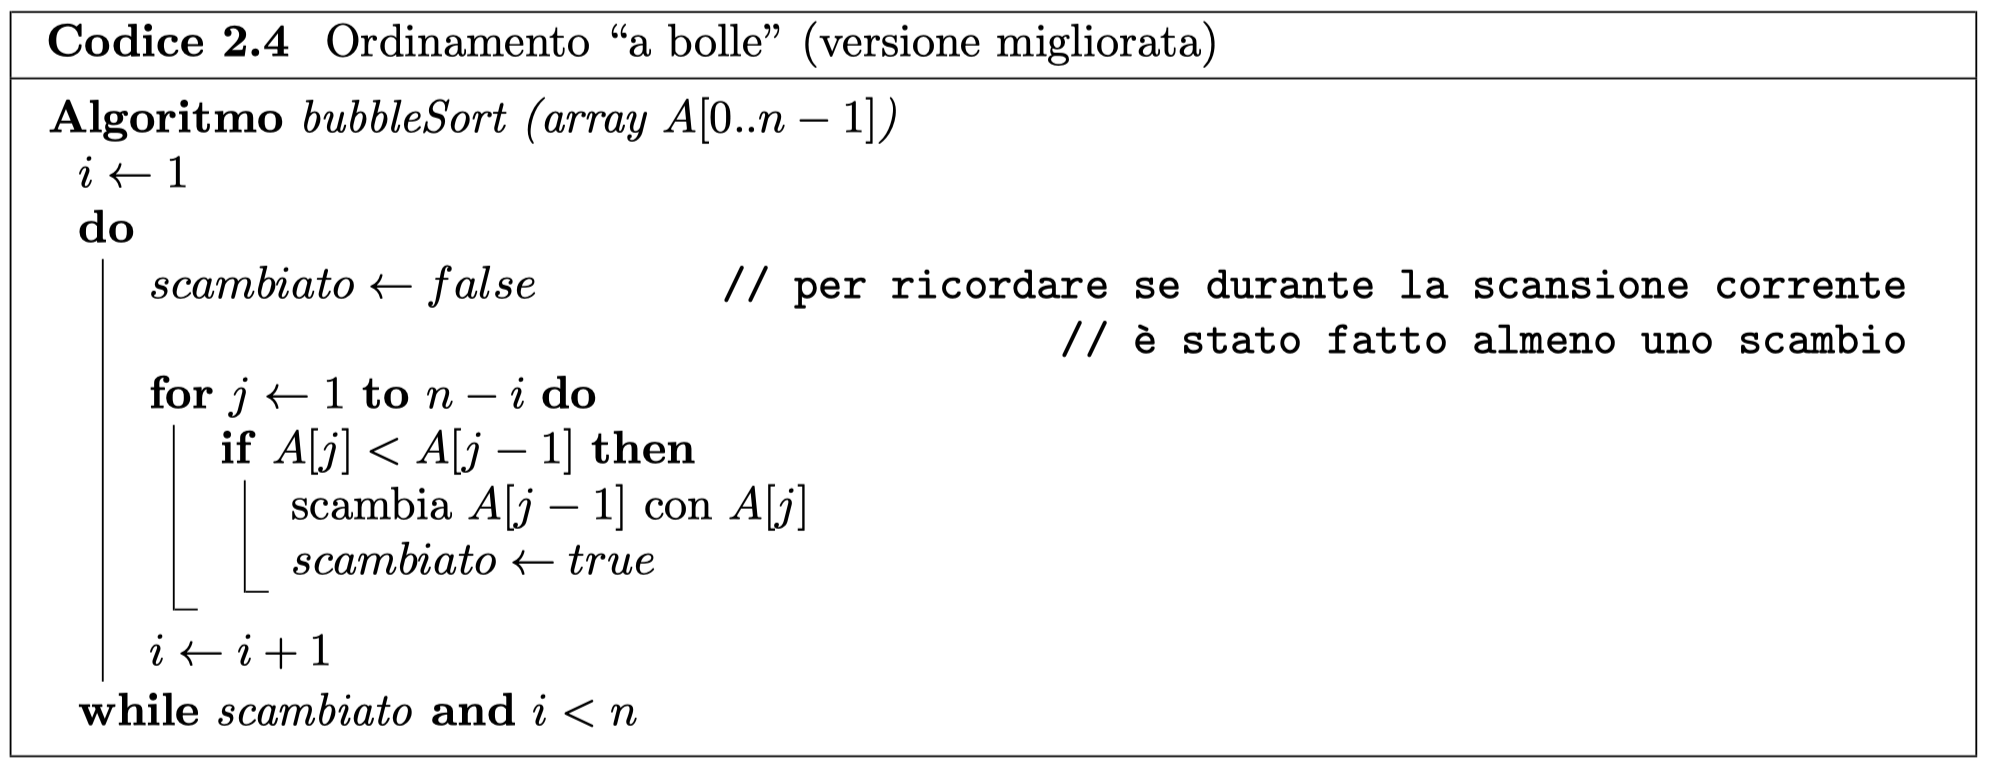
\includegraphics[width=\textwidth]{bubblesortmigliorato.png}
\end{figure}

\subsubsection*{Esempio di esecuzione versione migliorata}
\begin{figure}[h]
        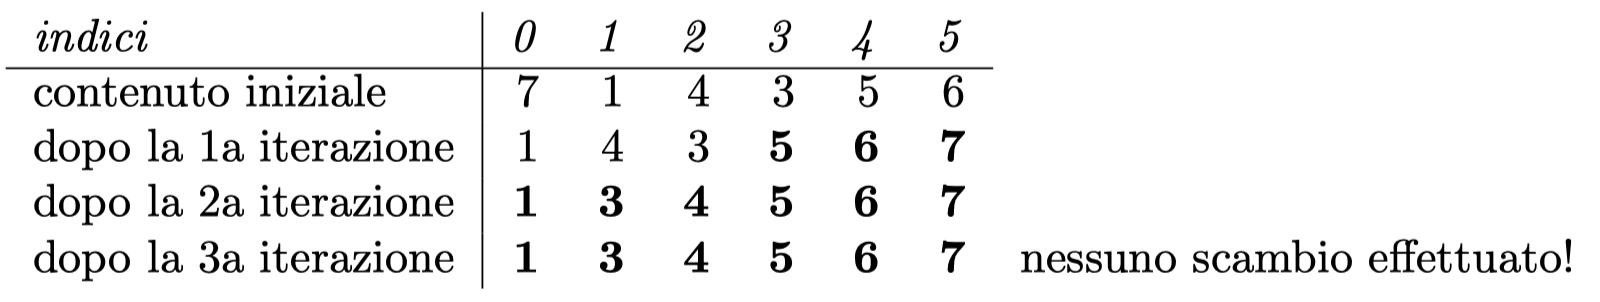
\includegraphics[width=\textwidth]{bubblesortexmigliorato.png}
\end{figure}

\subsubsection*{Numero di confronti}
Nell'iterazione $i$ del ciclo principale si effettuano esattamente $n - 1$ confronti.
Il ciclo principale viene eseguito a partire da $i = 1$, incrementando fino al più
a $n - 1$. Pertanto sommando su tutte le iterazioni il numero di confronti è al massimo $\frac{n(n-1)}{2} = \Theta(n^2)$
nel caso peggiore, che si ha quando l'array è ordinato al contrario.
Se invece l'array è già ordinato il numero di confronti è $n - 1$ 

\subsubsection*{Spazio}
L'algoritmo, oltre all'array da ordinare, utilizza un numero costante di variabili.
Pertanto la quantità di spazio aggiuntivo è costante.
\clearpage

\subsection{Una considerazione su confronti e spostamenti}
Abbiamo detto che la stima del tempo di calcolo di questi algoritmi 
può avvenire a partire da quella del numero di confronti, 
moltiplicando il numero di confronti per il tempo necessario per 
effettuare ciascun confronto. Questo è vero a patto che i confronti tra chiavi 
siano le operazioni più costose effettuate dagli algoritmi. 
Potremmo calcolare anche il numero di spostamenti di elementi. 
Da questo calcolo possiamo scoprire che tra i tre algoritmi presentati sopra, l’ordinamento per selezione
è quello che effettua un numero di spostamenti più basso. 
Ma quanto costano gli spostamenti in termini di tempo? Come per i confronti, 
se stiamo ordinando numeri interi di grandezza fissata, come i valori dei tipi {\texttt{int}} e {\texttt{long}}, 
gli spostamenti sono effettuati mediante assegnamenti che copiano un numero fissato di bit, e quindi avvengono in tempo costante. 
Se tuttavia, come avviene nella pratica, stiamo ordinando rispetto a un campo chiave dei record di grandi dimensioni, 
la copia di interi record diventa costosa in termini di tempo e il numero di spostamenti può essere un parametro critico, 
anche più importante del numero di confronti, per valutare il tempo impiegato da un algoritmo.
Questo problema può essere evitato utilizzando i puntatori: 
anzichè memorizzare negli elementi dell’array i record da ordinare, 
possiamo memorizzare i puntatori ad essi. 
Quindi, ogni cella dell’array conterrà il puntatore a un record, memorizzato altrove. 
In questo modo, per effettuare uno spostamento, non è necessario copiare l’intero record, 
ma solo copiare dei puntatori ai record. La dimensione dei puntatori può essere considerata costante 
(dipende dalla grandezza delle memoria che può essere indirizzata).
\clearpage